\section{Investigation of the Current System}
This section details the in-depth investigation that was performed on the current quiz system used by the school. Initial contact with the school was made via an email to one Mr Nick Bucknall, currently head of Year 8, on the 30th June 2015. Following a brief email exchange, the details of which can be found below, Below can be found the different aspects that were investigated.

% \subsection{Overview of System}
% Currently, the school does not have a formal, standardised system in place. A somewhat ad-hoc approach is currently used, using a combination of emails, documents scattered across the network, and verbal communication. Obviously, this approach has a number of issues, the details of which can be found below in the observations performed, as well as the analysis of the current system's limitations.

% Import interviews
\subsection{Interviews}

A number of interviews were held with staff at the school. Two form tutors were interviewed, in order to gain an insight into how they believe form times could be improved through the use of interactive quizzes, and to get an idea of how they would like such a system to work. Additionally, Nick Bucknall, a head of year at the school, was interviewed; he was chosen in order to gain information on what results the system should calculate, and how best to integrate such a system within the school. He was also chosen to get a further idea of the faults with the current system. Full transcripts for each of the interviews are included below. In addition to the formal interviews held with teaching staff, two informal meetings were held with other key members of the school community - Tim Alexander, one of the IT technicians in charge of the school's network, and Michael Barratt himself. Due to the length of these meetings and the unwillingness of the participants to be recorded, full transcripts are not available. Instead, notes on the key topics covered have been listed below.

\subsubsection{Bryan Warr}
\textit{\textbf{DR:}} So what would you say is the main focus of form time?

\textit{\textbf{BW:}} Okay. So, there's several different types of form time. One could be focusing the students on silent reading, one could be on numeracy, one could be on literacy, another could be on a discussion - on something moral or spiritual. Obviously we've got assembly time as well, but it also depends on the audience - it depends on whether they're Year 7 or whether they're Year 11. So for Year 7's it would be different to Year 11's. For example, Year 11's might spend time revising, or focusing on exam technique; but Year 7's, a lot of time is spent with Year 7's building up the relationship with their tutor. So some of that could be activities that get them all working together.

\textit{\textbf{DR:}} I see. How important is that during the later years?

\textit{\textbf{BW:}} Yeah, it's still important, definitely. I suppose it depends on whether your tutor is new or not - you might have a tutor who's newer to Year 10 or Year 11, and wants to spend their time getting to know them. If you've had a tutor that's taken you all the way through, like my tutor group, then you don't need those ice breakers as much - you know each other quite well.

\textit{\textbf{DR:}} And how often does it occur that form teachers leave halfway through?

\textit{\textbf{BW:}} Here it's not very often. It's not as often as it is in other schools - in some schools it's all the time. My last school, I took a group through Year 11, and it was unusual, because every single tutor in that year group was with them from Year 7 to Year 11, which is very rare. But here for example, our Year 10 tutor group, pretty much similar tutor team from the start to the end. There's been a little change - so tutors do change, but there's always a set activity list from the head of year, head of house I should say.

\textit{\textbf{DR:}} So does the head of year have more control than the individual form tutors?

\textit{\textbf{BW:}} Yes. The form tutor is told by the head of year, well next year it will be the head of house, what to do. So we get given a timetable, it's on the wall, we get given a tutor program. Do you wanna see one?

\textit{\textbf{DR:}} Yeah, that would be helpful.

\begin{center}
\textit{\textbf{* DR and BW move to the classroom wall, to look at the timetable *}}
\end{center}

\textit{\textbf{BW:}} So these change every year. This is the Year 10 one - this is the summer one.

\begin{center}
\textit{\textbf{* Microphone fails to pick up conversation for the next 30 seconds. BW prints out tutor timetables for Year 9, Year 10 and Year 11, available below. BW and DR sit back down again. *}}\\
\end{center}

\textit{\textbf{BW:}} So you'll see that that one's key stage 3, and then you've got Year 10 and Year 11. So is you're idea maybe that you'd trial it here, or were you thinking...?

\textit{\textbf{DR:}} Yeah. The thing we've got to do is think of an idea for a system, and then go to a business - in my case it's here - and do interviews, with people who would use the system; hand out questionnaires, and perform observations. I've done my observation because I just used my experience here, and I'm doing interviews now.

\textit{\textbf{BW:}} So, Mr Bucknall would be a good one to talk to.

\textit{\textbf{DR:}} I've arranged one with him.

\textit{\textbf{BW:}} He's a head of house next year. So he's obviously, he's directly - he writes that. So the tutors, heads of house, who else? Also SLT, any members of SLT - I'm on SLT next year as well. Obviously the assemblies are run by members of SLT, but you can see there's a theme running through them - Year 9, you've got literacy, numeracy, in each one; you've got group discussions or activities, you've got silent reading in each one, because it just needs to be established. In Year 11, that would be revision, or personal study. And in Year 10 we give them that opportunity as well - we say, ``right, if you want to study, you do that.'' It's a lot more open than in Year 7.

\textit{\textbf{DR:}} The idea I had focuses mainly on the quiz aspect - automating it, so to speak, and making it more competitive. How do you feel about quizzes? I can see they're fairly regular on the timetable, but less so in Year 11.

\textit{\textbf{BW:}} Well, Miss Mitchell used to do them, and she was quite good at them. The quizzes are...I find them a bit hit and miss, on my own quizzes. The Year 10's do like them, my Year 10's. If they were automated, that would work. And if it was a competition between houses...

\textit{\textbf{DR:}} Yes, that's what I was thinking.

\textit{\textbf{BW:}} That's what we're...that would be really...I would have thought that would be quite well received, because obviously we're moving towards bigging up the house system next year.

\textit{\textbf{DR:}} Okay.

\textit{\textbf{BW:}} So the house system is going to be more prevalent, so the fact that you're competing into forms...and also, heads of house would like it, because you've halved their workload, if a quiz is being laid on every week, definitely would be useful. It's obviously going to be difficult that you've got 7, 8, 9, 10 and 11...

\textit{\textbf{DR:}} All of whom need doing.

\textit{\textbf{BW:}} With different quizzes. That wouldn't be too difficult.

\textit{\textbf{DR:}} No. So, when I was in Year 11, Mr Bucknall seemed to control the quiz system quite heavily.

\textit{\textbf{BW:}} Yep.

\textit{\textbf{DR:}} So he'd make the quiz himself.

\textit{\textbf{BW:}} Yes, that's right.

\textit{\textbf{DR:}} And then handed out different quizzes. How do you feel about that, if that's what Mrs Shaw does with you?

\textit{\textbf{BW:}} Happy with that. If it was centralised, it would be even easier. So if the heads of house didn't have to handle that, if it was in a central system, that you could access, that would be easier.

\textit{\textbf{DR:}} So say there was an icon on the desktop, that opens up the program, showing the quiz for the week.

\textit{\textbf{BW:}} Yes. Perfect. And if you chose Year 7, with a choice of the year groups, that would be easy. So the tutor could say ``right, I want the Year 7 one to come up'', that would be perfect. Yeah.

\textit{\textbf{DR:}} Because what I was thinking was the different heads of year, or houses now...if they wanted a quiz, they'd write it using the system, and then they'd have access to their form groups, so then they could target...and then they could send it that way. Would that be something they'd be interested in?

\textit{\textbf{BW:}} Possibly, but don't forget that now they're heads of house...so Mr Bucknall, who's got Darwin, he's now got five years. So again it's the same issue, each head of house has got to make lots of quizzes.

\textit{\textbf{DR:}} So, there aren't heads of year anymore, there are houses?

\textit{\textbf{BW:}} Right. So we've got Acton, Baxter, Clive, Darwin, Houseman and Webb; and then each one's a house with a vertical setup to it.

\textit{\textbf{DR:}} I see.

\textit{\textbf{BW:}} So you're going to have the same issue with each one, in that they've got to differentiate between the years. And what they wouldn't want to do is replicate their work. So I don't think they'd be happy if they were...say Mrs Smith was doing this, and she had to do all the years, and Mrs Heath had to do the same, that would be a lot of repetition, whereas we could probably do the same...you could do the same thing for each one, couldn't you? If you did Year 7, just...bam. Year 8...right, just like that. That would be more sensible.

\textit{\textbf{DR:}} Okay. So, with assemblies and such, are the heads of houses taking each individual house each week? It wouldn't be say Mr Bucknall who speaks to the whole of Year 11 on a Tuesday?

\textit{\textbf{BW:}} Occasionally there will be a need for us to speak to Year 11 or Year 10 to do with certain aspects. But the majority of assemblies are with the houses, so it would be Mr Bucknall talking with Darwin - all the years. Okay? So it will be a house assembly. And we have whole school assemblies now on Mondays, first Monday of the month, which Mr Barratt does. So that's every Monday, and it's whole school, in the sports hall.

\textit{\textbf{DR:}} Kind of like it was at the end of term before?

\textit{\textbf{BW:}} Exactly, yeah, yeah. He's got it every month now, so we get together as a whole.

\textit{\textbf{DR:}} Right. So how do you feel...if the school's looking to improve cooperation between houses, how would you feel about that taking place in form time?

\textit{\textbf{BW:}} How do you mean?

\textit{\textbf{DR:}} Well, if, say, there was the quiz, say on that side of the screen, and on the other side was a view showing how the other forms are doing, in real time, would that be something you'd be interested in?

\textit{\textbf{BW:}} It could be interesting, yeah. Could be interesting. Definitely brings in the element of competition, live, rather...

\textit{\textbf{DR:}} Yeah, because that makes it a lot more interesting, than finding out say a week after that Baxter has won.

\textit{\textbf{BW:}} The only problem you've got is that they wouldn't necessarily be the same years on the same days.

\textit{\textbf{DR:}} How do you mean?

\textit{\textbf{BW:}} Well you'll have Acton...you're Year 7 quiz could be on the same day, but Year 7 and Year 10 might not be. Because the tutor programs are different, because they have to be, because of the assemblies and rooms, so for example the KS4 assembly there is on a Tuesday, but there it's silent reading. So they could be doing a quiz, but these lot could be in assembly. So there could be a house assembly on, when you've got Acton doing it. So, you'd have to look...

\textit{\textbf{DR:}} But horizontally, that wouldn't be an issue.

\textit{\textbf{BW:}} Right, horizontally, it would work, yeah. All of Year 7 would be together at the same time, unless there's a house assembly - if there's a house assembly on, it means that house would be out. So you'd have to look for where there's that literacy or numeracy activity, or something like a silent reading activity, where there's something with a group discussion. But I'm sure the heads of house wouldn't mind if, once a month, one of those...you'd have to ask Mr Bucknall of course, I'm sure he wouldn't mind...if one of those was taken up with a house quiz. Because if you did that, I'm just thinking...within a half term, you could get one quiz in for every year group. You could take one silent reading or one literacy or numeracy activity, and replace that with a house quiz, for the year group, that would work.

\textit{\textbf{DR:}} Okay. And what sort of topics would the quizzes best fit? Because when I did them, it kind of varied each week, so sometimes it would be culture, sometimes it would be general...stuff.

\textit{\textbf{BW:}} General knowledge is always good. Music's always good. Popular culture. Anything like that you could have. You could make it so they were subject related. So you could have history, geography or maths.

\textit{\textbf{DR:}} Right. So how would you, as head of maths, feel about there being a maths quiz?

\textit{\textbf{BW:}} Yeah. I'm happy with that. We're doing inter-house competitions within the subject, so we're going to do a Countdown activity. But I'd be absolutely fine with that, a maths quiz now and again, because again, it raises maths in the school. I'm sure the other heads of department are the same.

\textit{\textbf{DR:}} Okay. Trouble is trying to make it seem like a quiz, rather than a test, which I guess it would be.

\textit{\textbf{BW:}} Exactly. And also, you've gotta be careful with differentiation, because some students are much better at maths than others.

\textit{\textbf{DR:}} So would the top group have done things that the lower groups would have done?

\textit{\textbf{BW:}} Yes. Yeah, they'd have done some different things, so...maths quiz. See, my tutor group's a good example. I've got a tutor group where I've got some brilliant mathematicians, and some who really struggle, and to give them maths quizzes is always difficult, because some are at an advantage straight away - even with Countdown they're at an advantage. That would be a tricky one. General knowledge is probably better because everyone can access that. I mean, even if you did a History quiz, some people would be at an advantage. That's a tricky one. You could make it so that it would be subject related quiz, on a one off, where there was bits of Maths, bits of History. I suppose you could do that, make it more general.

\textit{\textbf{DR:}} Yeah, cause each form has people who are good at some things...

\textit{\textbf{BW:}} That might make it more accessible.

\textit{\textbf{DR:}} And how well would it work? If the form had to work with one another, to work out the answer?

\textit{\textbf{BW:}} That would be fine. Yeah, it wouldn't be an issue. The forms are used to working together.

\textit{\textbf{DR:}} And are all forms going to be happy working that way? Certain forms and year groups, I imagine, are less likely to work well with that sort of system.

\textit{\textbf{BW:}} Depends on the form tutor really. But the majority of the time, the form tutors accept what's asked of them. Certainly the majority of cases.

\textit{\textbf{DR:}} And how would participation be dealt with? There'd be some people at the back of the room who don't participate.

\textit{\textbf{BW:}} Right. You could do...to ensure participation, could be something like use the iPads. You could do something either...we do work using Socrative, using that. It's an app where everybody has to answer. So, I set the Socrative quiz up recently with my Year 7's. It's a web based one, so something like this would work. So with Socrative, I set a quiz up for the Year 7's, and you can see the live results come in. What they do is they can login to your room, and the quiz comes up as you're doing it - you get live results, with a load of reports. So I've got these results here, and these have all come through, and that's how it comes through. So there's the questions and answers - I can see that who's answered, and as they were doing it, I knew that Izzy hadn't done it. So maybe something like that would ensure participation.

\textit{\textbf{DR:}} So this is kind of like the old Quizdom system they used in Science.

\textit{\textbf{BW:}} Quizdom, exactly.

\textit{\textbf{DR:}} I never thought that worked very well.

\textit{\textbf{BW:}} No, these work a lot better - there's less faffing about. It's a web based system, so the room is accessible to anyone - it's constant; that will always be my room, whatever quiz I do. But that would work. Other than that, you're sort of relying on the teacher just...getting everybody involved.

\textit{\textbf{DR:}} Is that something the school is looking at - raising participation - or is that not really an issue?

\textit{\textbf{BW:}} We're looking at raising participation with the house system, and anything that does that is going to be useful. I don't think engagement in general is a problem in this school.

\textit{\textbf{DR:}} So if this sort of system were implemented in form time - purely in form time - would that be an issue, or should it be expanded for use in subjects?

\textit{\textbf{BW:}} I think it would be useful in form times to start with. Purely to address the problem the heads of house have. It also makes it more unilateral, doesn't it? Yeah, I think that would work.

\textit{\textbf{DR:}} How technical would you say that you are?

\textit{\textbf{BW:}} I'm pretty good. No, I'm not too bad. I can deal with most things, but not everybody's the same.

\textit{\textbf{DR:}} No. I'm trying to make it as simple as possible - thinking of people like Mrs England.

\textit{\textbf{BW:}} Yeah, some people would struggle. So it literally needs to be...two clicks. One click to get into the program, click to choose your year, maybe another to start the quiz.

\textit{\textbf{DR:}} How would you feel about a login system, where you had to sign in?

\textit{\textbf{BW:}} A login system would be fine. It would prevent the students hacking it.

\textit{\textbf{DR:}} Yeah, that's what I'm thinking.

\textit{\textbf{BW:}} Yeah, that would work. We're used to logging in to stuff. So yeah, happy with that.

\textit{\textbf{DR:}} This sounds a little crude, but would you be tempted to help your form in any with, if there was a reward for the best performing house?

\textit{\textbf{BW:}} Right. Are you suggesting would I cheat?

\textit{\textbf{DR:}} Yes.

\textit{\textbf{BW:}} Right. No, it's a good question. No, I wouldn't help them with it. I don't think they'd need my help - they work quite well together. I'm not convinced that every teacher would feel the same. \textit{\textbf{*laughs*}}

\textit{\textbf{DR:}} Okay. And is that going to be different depending on their year group?

\textit{\textbf{BW:}} Possibly, yeah. For Year 7 we'd approach it differently to Year 11.

\textit{\textbf{DR:}} And how suitable would this be if the school had, say, a theme of the term or theme of the week?

\textit{\textbf{BW:}} They do come up, but they would be more weekly things - so sometimes you have Anti-Bullying Week, or Global Entrepreneurship Week - so they come up now and again.

\textit{\textbf{DR:}} I see. And would this system come in useful for the quiz aspect of that?

\textit{\textbf{BW:}} Yeah, absolutely. And I'll tell you who else would be interested in this as well: Mrs Hancox and Miss Morris who run Life. Life would be really interested in this. I'm just thinking outside the box, purely because Friday lesson 2, when you have Life, you would have all of the year group in the same lesson at the same time - everybody in the school. So there might be an opportunity in Life as well.

\textit{\textbf{DR:}} I'll send them an email I think, thank you.

\textit{\textbf{BW:}} That might be worth talking about. You know...did Miss Hancox or Miss Morris teach you?

\textit{\textbf{DR:}} Miss Morris taught me for three years, yes.

\textit{\textbf{BW:}} Right, so you know her. So they're the heads of Life - they'd be interested in this, and that would be a good opportunity to use it, potentially. And with Life, they've got all sorts of things, so there's a lot of opportunity for quizzes.

\textit{\textbf{DR:}} If this were rolled out, how likely is it that it were actually used?

\textit{\textbf{BW:}} I think if people are told to use it, they'll use it.

\textit{\textbf{DR:}} Okay. And how would the heads of house tell you?

\textit{\textbf{BW:}} When I get this from Mrs Shaw, I follow that, because she tells me to. We know what we have to do - this on a Monday, that on a Wednesday. It might not be that we do the same thing, but we do some literacy and numeracy, then we do a group discussion or quiz, and then we have assembly. So we have that programme, and we follow it. We're actually checked up on whether we do that. SLT will check, randomly - we don't know when they're coming, but it's with the head of house, and they check what you're doing. If you're not doing what you're meant to...trouble.

\textit{\textbf{DR:}} Right. I remember last year, I had Mr Massey. And he wasn't...

\textit{\textbf{BW:}} \textit{\textbf{*laughs*}} You don't have to say any more!

\textit{\textbf{DR:}} And that was an issue sometimes.

\textit{\textbf{BW:}} Yeah. Okay. I feel your pain. \textit{\textbf{*laughs*}}

\textit{\textbf{DR:}} So, how would you feel about the quiz...

\textit{\textbf{BW:}} \textit{\textbf{*laughs*}}

\textit{\textbf{DR:}} About the quiz...\textit{\textbf{*laughs*}}...not starting until all the teachers had signed on?

\textit{\textbf{BW:}} Yeah, happy with that. I mean, it could be that you could trial it with one year group. You could ask the heads of house which year groups they feel most confident about giving it to. It might be that you've got a team of tutors in that year group who know they kids better, who've been together longer, who are maybe more confident dealing with this stuff, before you roll it out. Don't forget, you've got Year 7 tutors coming in September, who are gonna have to get to know their tutor groups. That'll be the priority for them. Year 11, pretty much starting them on exam technique...well, with the exception of your tutor \textit{\textbf{*laughs*}}. You want to get the ball rolling and get them into exam mode, so maybe a Year 9 team...\textit{\textbf{*laughs*}} yeah.

\textit{\textbf{DR:}} Sorry. \textit{\textbf{*laughs*}}

\textit{\textbf{BW:}} I dread to think! \textit{\textbf{*laughs*}} Who was in your tutor group? Name me some interesting characters.

\textit{\textbf{DR:}} Nick Porter.

\textit{\textbf{BW:}} Jesus. Right. Go on.

\textit{\textbf{DR:}} Doug Coull.

\textit{\textbf{BW:}} Oh right, not too bad.

\textit{\textbf{DR:}} Liam Davies.

\textit{\textbf{BW:}} \textit{\textbf{*laughs*}} Say no more - we're there!

\textit{\textbf{DR:}} \textit{\textbf{*laughs*}} So how would you feel about an email in the morning, reminding you of the quiz? Obviously you've got the timetable, but not all teachers are going to follow that.

\textit{\textbf{BW:}} \textit{\textbf{*laughs*}} Yeah, emails would work. Most of the teachers check their email in the morning.

\textit{\textbf{DR:}} That wouldn't be seen as too overbearing?

\textit{\textbf{BW:}} No, I don't think so. You could also set up a reminder on Outlook - that would work. Rather than an email, we could get a reminder, at whatever time the quiz is supposed to take place, so my Outlook is linked to my calendar. I get a reminder and it would just say ``Year 10 quiz - 1:40pm''. That might work as well.

\textit{\textbf{DR:}} Well, I think that's pretty much it.

\textit{\textbf{BW:}} Okay.

\textit{\textbf{DR:}} But thank you very much, you've been very helpful.

\textit{\textbf{BW:}} Anytime! I would set up a discussion with the heads of house - certainly Mr Bucknall.




\subsubsection{Wendy Blower}

\textit{\textbf{DR:}} So, my project is...I've got to come up with a system for a business, in this case Priory. It's to do with form times - a sort of quiz system, an automated one. The heads of house could write a quiz, and send it out to the different house groups, for it to be answered in form. The results would be calculated, reports made, etc. That's just a basic overview - what are your thoughts?

\textit{\textbf{WB:}} It sounds like a good idea to me. If I can just clarify exactly what it is...so, during tutor time in an afternoon, I'd be told that there's gonna be a quiz, that would all be online...

\textit{\textbf{DR:}} Yes.

\textit{\textbf{WB:}} So then we'd do it as a form...

\textit{\textbf{DR:}} Yes.

\textit{\textbf{WB:}} We'd put our results into the system...

\textit{\textbf{DR:}} Yes.

\textit{\textbf{WB:}} And then somebody, one of the heads of house, could log into a system and see, well, 8A got this many, 9A got this many, or whoever...Yeah. I think that sounds like a great idea.

\textit{\textbf{DR:}} Alright, so...I'm sorry, I've got so many questions...

\textit{\textbf{WB:}} That's alright, don't worry!

\textit{\textbf{DR:}} So would you prefer the system to be the form working together as a whole, or with each individual student, perhaps with an iPad?

\textit{\textbf{WB:}} Right, I can see ads and disads to both. From an efficiency point of view, I think if it was the whole form...I think there would be less mistakes that could be made. Because then it's either the member of staff at the computer, or one student with an iPad, and then everything gets done in one go. If you then had each student with an iPad - which I think the students would prefer, because it's more fun - if a student doesn't bring their iPad with them, or it's dead, or...not everybody has one so we have to get some from IT, what happens if we can't book them? I know you could book ahead, so I think I would prefer it if it were just done centrally...although maybe if their was an option to do either, that might be good, because their might be some days where I know I can book iPads, and I know everybody's got one, so I might say ``right, today, you're all going to do it on your own iPad''. So it's a bit like...did you ever use...

\textit{\textbf{DR:}} Quizdom?

\textit{\textbf{WB:}} That's the one! I was thinking Quizlet and that didn't sound right. Yeah, Quizdom - it sounds a bit like that. Is that the kind of thing you were going for?

\textit{\textbf{DR:}} Yeah. But I probably couldn't do both.

\textit{\textbf{WB:}} Right, okay.

\textit{\textbf{DR:}} Because it is all quite complicated, and it does take a while to...

\textit{\textbf{WB:}} Is there one that's easier than another? From your point of view.

\textit{\textbf{DR:}} Yes, the one with iPads would be quite a bit harder - but it would be more rewarding.

\textit{\textbf{WB:}} Oh, God! Okay, so if I had to go with one...who is this, who is it supposed to benefit? Is it supposed to be about engaging students?

\textit{\textbf{DR:}} Yes. I was told by Mr Warr that the school is trying to focus on the house system.

\textit{\textbf{WB:}} Yeah. I think if your aim - if your main aim is about engaging students, I think you'd have to do it with the iPads. Where they each have their own iPad, feeding to a system. I think us doing it, one feeding into one thing...perhaps if the aim was more about collating points in an efficient way, maybe that. So I think it's gotta do with your aims, hasn't it? Whatever your aim is, you have to pick the one that's suited more to that. Does that make sense?

\textit{\textbf{DR:}} Yeah, absolutely. What I thought would be nice if each student gave an answer to the quiz, and then the most popular answer in that form became that form's answer, but then if that's spread across 7A, 8A, 9A and so on, the most popular answer out of those becomes that house's answer.

\textit{\textbf{WB:}} Right, I see. But then would you need all of 7A, 8A, 9A and so on - would we all have to do the quiz at the same time?

\textit{\textbf{DR:}} Yes - and that's what I was speaking to Mr Warr about: getting the right time. With the form timetable, he says there could be a slot each term, where that could be done.

\textit{\textbf{WB:}} And I think that's the thing actually - with him saying each term, I think that would work, if we knew that...I don't know, on a day in October, and a day in January, and a day in say April...if we all knew, then yeah, I think it would work. But, see, we used to have a quiz on our timetable once a week. So I suppose in my head I was thinking that we'd be doing this once a week - it just wouldn't work, because things crop up, and then somebody gets called out, whereas if everybody knows that on this particular date everybody's gotta be doing it, then I think it could work really well, and I think that would be another reason why everybody should then...hold on, I've just thought of another problem...that's why everybody should then do it on their iPads, because they'd be like ``oh yeah, we wanna beat them next door'', because everybody would be doing it. But, if we all did it at the same time, there wouldn't be enough iPads.

\textit{\textbf{DR:}} That's what I wasn't too sure about. Because, I'd heard the school has an iPad loaning scheme. How widespread is that?

\textit{\textbf{WB:}} At the moment, we've got...I think it's approximately half of Year 8 have got them, and approximately half of Year 9. As far as I'm aware, I think that will happen...so this Christmas - this is how we did it last time - this Christmas, it will then be launched to current Year 7's, because they'll be Year 8 again. So ultimately, in a couple of years time, there will be at least half a year group in every year would have an iPad. So it's whether you could do it where, if it would work like this, it might be that you say ``right, on Thursday, everybody in A, and everybody in B does it''. So 7, 8, 9, 10, 11, A; 7, 8, 9, 10, 11, B. I mean, I'd still have to work out how many iPads that is, but it's whether you could do A and B on one day, C and D, H and W. If you could do that, we'd then have enough iPads. Could you still get it to work?

\textit{\textbf{DR:}} I think I probably could do, yes.

\textit{\textbf{WB:}} Right, okay. Or even if you...could you do just all of Acton on one day? If there wasn't enough iPads?

\textit{\textbf{DR:}} See, I suppose you could do, but what I really wanted to focus on was the realtime nature...

\textit{\textbf{WB:}} Oh right. Yeah...

\textit{\textbf{DR:}} So you'd have a thing at the bottom saying ``Webb has chosen this answer''...

\textit{\textbf{WB:}} Right, I see.

\textit{\textbf{DR:}} ``Three quarters of Houseman have now answered'' - it just makes it more interesting.

\textit{\textbf{WB:}} Oh, okay. Did Mr Warr say anything about like...the number of iPads that we've got available?

\textit{\textbf{DR:}} No, I haven't spoken to him about that.

\textit{\textbf{WB:}} Right, because...is it only me that you're talking to about it, or have you got people...?

\textit{\textbf{DR:}} No, I'm speaking to Mr Warr, you, Mrs Smith, Mr Bucknall, and the IT guys [Tim Alexander].

\textit{\textbf{WB:}} Right, okay. So in fact...it might be the IT guys might be able to help you out a little bit more there - because they know exactly how many iPads we've got. Yeah, that's more the technical side then, isn't it? But yeah, I agree actually - if you're focusing on the real time...I mean, I've been in a school before where we did...it was a talent show, and everybody scored at the same time. I can't even remember how we did it, but everybody scored at the same time, so you know like you see it on the TV? When you look on the screen, and it's like ``who's voted for person A'', and all the scores start going up, and you all vote at the same time.

\textit{\textbf{DR:}} That's kind of what I had in mind.

\textit{\textbf{WB:}} Yeah. So I see how that would be so good, and everybody would love it, to be able to see...yeah. So the IT guys are your best bet for talking about it. I mean, how long do you think this would take to make?

\textit{\textbf{DR:}} Well, the coursework officially has to be finished by the end of the Easter term. By that point, I should have a mostly working, fully tested system, but I'll need to do a bit of extra polish and work out a deployment strategy with the IT guys before it's ready for the school to use.

\textit{\textbf{WB:}} Okay. So I think in terms of real life then, if we were going to use this moving forward, we're at least a year away then, aren't we? By which time we might have more iPads. I mean, I'm looking at getting rid of all my laptops, and replacing them with iPads, and that certainly can't be done by tomorrow. So it might be we've got more iPads in school by then anyway, so it might work.

\textit{\textbf{DR:}} And bear in mind, in Mrs Smith's and Mr Edge's rooms, they can use the computers, because it would be web based.

\textit{\textbf{WB:}} Oh, so we could use the computer rooms, like 22 and T1?

\textit{\textbf{DR:}} Yes.

\textit{\textbf{WB:}} And then of course we've got laptops in school. Oh, okay. Okay, yeah. You're idea is good then, that it's the real time.

\textit{\textbf{DR:}} So, how well do you think students would take to this sort of system? I did the quizzes last year, just on paper, and I never thought it was that much fun.

\textit{\textbf{WB:}} I've got a Year 8 tutor group, and I think they would love it. Have you thought about talking to any students?

\textit{\textbf{DR:}} I emailed Mrs Smith a questionnaire to hand out, but I haven't heard back yet.

\textit{\textbf{WB:}} We have got a Year 10 student you could ask in the room...

\textit{\textbf{DR:}} That could be very helpful.\\

\begin{center}
\textit{\textbf{BETH, a Year 10 student, joins the interview.\\}}
\end{center}

\textit{\textbf{\\WB:}} Beth!

\textit{\textbf{BETH:}} Yes?

\textit{\textbf{WB:}} I'll try and talk a bit louder so you can hear me on your ear phones. Right, just picture it. You know when you've done quizzes in form time before, and it's a piece of paper, or your teachers reading out a quiz, imagine that scenario in your form room. How does everybody feel about it? Are you bored? Do you like it? Does everybody get involved?

\textit{\textbf{BETH:}} Not really.

\textit{\textbf{WB:}} Do you know the reason why?

\textit{\textbf{BETH:}} It's just quite boring. The questions aren't very good.

\textit{\textbf{WB:}} Okay. So imagine the same questions - pretend the questions are the same - but this time, you're all voting for answers via...would it be an app?

\textit{\textbf{DR:}} Yes.

\textit{\textbf{WB:}} Via an app, or you're on a laptop doing it, and the whole school's doing it at the same time. So you do it in your house - who's your house?

\textit{\textbf{BETH:}} Webb.

\textit{\textbf{WB:}} So you'd be doing it for Webb, and real time you would be able to see on the board what everybody's answered, and who's winning?

\textit{\textbf{DR:}} Yes.

\textit{\textbf{WB:}} Would that make you more...want to do it more?

\textit{\textbf{BETH:}} I think so, yeah. I've got quite a competitive form, so if we could see our results live against the other forms, that would make it a lot more interesting.

\textit{\textbf{WB:}} Right. Is that from me saying that you're competing with everybody else, or would it help that it's real time and you're using apps and stuff?

\textit{\textbf{BETH:}} I think it's more that we can see what everyone else is doing, and that it has a bit more importance. At the moment they just get thrown in the bin. But if it's for house points and actually matters, then that would be better.

\textit{\textbf{WB:}} Right. So your age group...'cause I'm just saying to Dee here that my tutor group are in Year 8, and I know they'd love to do that, where they've got apps and they can answer. I know they'd love it, but of course they're a couple of years younger than you. So you think the competitive...

\textit{\textbf{BETH:}} Yeah.

\textit{\textbf{WB:}} It doesn't matter though that you'd be in Year 11, you'd still want to do it?

\textit{\textbf{BETH:}} Yes, if it's competitive enough.

\textit{\textbf{WB:}} Okay. Thank you!\\

\begin{center}
\textit{\textbf{BETH leaves the interview.\\}}
\end{center}

\textit{\textbf{\\WB:}} Sorry, I feel like I'm taking over the interview! \textit{\textbf{*laughs*}}

\textit{\textbf{DR:}} No, it's good! \textit{\textbf{*laughs*}}

\textit{\textbf{WB:}} \textit{\textbf{*laughs*}}

\textit{\textbf{DR:}} Should the individual tutors be able to help make the questions, or should that be left down to the heads of house? Before, with the head of year system, this would have worked a bit more nicely, because there's one key figure per year, but...

\textit{\textbf{WB:}} Hmmm. Good question. I don't think form tutors should be involved. I think we could be involved in...say like Beth's just been saying, they'd have like the questions, so it might be nice if, lets say...so I'm in Acton, so it would be good if in an Acton meeting, so there's like me, Mr Warr, Miss Jebb, Miss Hayman; and a new guy, who'll be starting in September; so there's the five of us and Mrs Smyth, she's head of house...it would be good if in a meeting we could say ``right, can we make sure that we've got...a section on history, a section on reality TV'', that kind of thing, so it's not all...like some of our quizzes, like Beth said, some of them are a bit boring. I don't know where the questions come from, whether they've just been taken of the internet, but they're a bit boring. So it'd be nice if we could have an input like that, but I wouldn't wanna have an input in the questions, because I know I wouldn't cheat \textit{\textbf{*laughs*}}

\textit{\textbf{DR:}} I see \textit{\textbf{*laughs*}}

\textit{\textbf{WB:}} Right! But of course, if I've got my form and they're all getting excited, it would be very hard to not guide them in the right direction, and I think it then would be unfair. Whereas if the heads of houses had come up with the questions, they could all be in their office, watching real time what's going on, and shouting at the screen! But they've got no input, and we didn't know what the questions were either, and it means we can get involved with what's going on, rather than it being them and us, kind of thing. We could get involved with them then.

\textit{\textbf{DR:}} That could be really good.

\textit{\textbf{WB:}} Yeah, because we're part of the house, you know, we're supposed to be joining in, with things that are going on, like, going off topic slightly, but there's a house run that's going to be happening, and we've got to do it as well. So... \textit{\textbf{*laughs}} ...I know! I'm not looking forward to that! But we can't expect them to do it if we're not going to do it. So it would be nice actually if we didn't know the questions.

\textit{\textbf{DR:}} Okay. And how would you feel if there were some subject related questions? I spoke to Mr Warr, and he said he wouldn't mind there being maths questions in there, but it's slightly different with business, because there's less of an ability gap.

\textit{\textbf{WB:}} I like the idea of there being subject questions...I think actually business could be alright, because all you'd have to do is make sure that there are only questions asked that you know students have studied in Years 7, 8 and 9. But then the only issue that brings up is if, if the form tutor is not supposed to know the questions, we'd have to have set them, wouldn't we? So...ooh, I don't know on that one. Be interesting to see what anybody else says. It depends what's more important - is it more important for tutors to get involved with their house, and try and work out the answers; or is it more important for us to ask questions around subjects? Like, on one hand, there's lots of questions you could ask in a quiz, but d'ya know what? History questions come up in quizzes more often than business. So there could be a history question that comes up, that is to do with something that they've learned. So unless we all had to put forward one question per department or something, and then we'd have to promise that we wouldn't give the answer out...\textit{\textbf{*laughs*}}...'cause otherwise we'd have an unfair advantage, when the business question comes up, and I'm the business teacher. So we'd have to just say ``right, I'm not gonna say anything for that''.

\textit{\textbf{DR:}} But, the subject questions could make it a bit like a test. I don't want to be rude, but business isn't the most exciting...

\textit{\textbf{WB:}} \textit{\textbf{*gasp*}} Dee!

\textit{\textbf{DR:}} Well it isn't though!

\textit{\textbf{WB:}} How dare you! But you did so well!

\textit{\textbf{DR:}} Not...amazingly well!

\textit{\textbf{WB:}} \textit{\textbf{*laughs*}} Okay, so then I think what you could probably do is if there was a business question, I possibly then wouldn't ask a business question that was about Years 7, 8 and 9, but I could ask a question about Richard Branson. So maybe, still do something from topics, that's more real life. I'm sure...could everybody else do that? I'm sure they could. Maths: what's the size of a football pitch? So maybe.

\textit{\textbf{DR:}} How easy should this be? The students in Year 7 aren't going to be able to cope with an overly detailed interface.

\textit{\textbf{WB:}} Are you talking about how easy the questions should be, or how easy to use?

\textit{\textbf{DR:}} Use.

\textit{\textbf{WB:}} In my mind, something like this is as easy as...a question, you know I'm thinking of apps I've seen before, a question, and multiple choices? Have you thought about whether it's gonna be multiple choice?

\textit{\textbf{DR:}} Yes, the people who make the quiz can choose between either multiple choice, multiple correct answers; or a custom input, where the students type in an answer.

\textit{\textbf{WB:}} I think it depends on the type of question as to whether you input yourself. So if you do both, I think some should be multiple choice...but let's say there was a maths type question. If the answer is like...15, or 1974, you can't type it wrong, can you? The answer is what it is. Whereas if you're asking someone ``what happened on the 7th July?'', however many years ago it was, the way somebody would write ``it was the day that London was bombed'', or whatever, everybody would write it differently.

\textit{\textbf{DR:}} But for that kind of question, multiple choice would be a better fit.

\textit{\textbf{WB:}} Yeah. So if you could do both, depending on the answer whether it would be multiple choice or just an open, I think that would be good.

\textit{\textbf{DR:}} Okay. And how quick are the iPads to get started with?

\textit{\textbf{WB:}} They're really quick. Do you mean in terms of using it in a lesson, switch it on, start using it?

\textit{\textbf{DR:}} Yes.

\textit{\textbf{WB:}} They don't get switched off. So literally, when they have an iPad, and when they've got their own iPad, they're all on. That's why we prefer them really. With the computers, well, you remember using them - they're a pain in the bum. You switch them on, wait for them to connect...it's not like that with iPads. So you could literally do it straight away.

\textit{\textbf{DR:}} Alright. And how long do you think the quiz should last?

\textit{\textbf{WB:}} I think it should be in rounds. I think if you're doing it...if it would be something that we would do once a term, I think it would be nice if the head would say that it's going to last longer than an afternoon's form time, for example. I mean, I've just presumed it would be done in form time.

\textit{\textbf{DR:}} Yes, that's what I was thinking.

\textit{\textbf{WB:}} So I'm thinking that we'd extend form till, I don't know, 2:15. I think if it's made a big deal out of, I think they'd really get into it. And I think rounds really spices it up. Like, I've done quizzes before, I don't know if I ever did one with your class, but I've done quizzes before where you've got the picture round, so you'd have a picture round and it gets passed round, but then you start with Round 1, and Round 1 is whatever, and Round 2 is whatever, and then you've got the music round as well. So I think it would be nice to do it like that. So I think different rounds...obviously we don't want it too long. Four or five rounds, maybe? And if it was finished and everybody started lesson 5 by 2:15, that then gives you...'cause you'd want to give the results as well. I know it's live, but...there's still got to be a certain element of us all going ``oh''.

\textit{\textbf{DR:}} Yes, I was thinking that could be done in the term assembly.

\textit{\textbf{WB:}} Oh yeah, that's a good idea. If you showed live things going on, if you showed ``well, Webb answered this and Acton answered this'', you're not telling us the answers at that point? Would some people work out who'd won?

\textit{\textbf{DR:}} That's a good point.

\textit{\textbf{WB:}} I mean it might be, you know like they do on ``Who Wants to be a Millionaire?'', where you know when you ask the audience and everybody presses the buzzers, and it's like ``this many people answered A, this many people answered B, C, D'', whether you could do it like that. The only other thing is...I think students would want to know the answer straight away. Beth, would you wanna know the answer straight away for the quiz or would you be happy to wait until an assembly?

\textit{\textbf{BETH:}} I'd want to know straight after I'd answered.

\textit{\textbf{WB:}} Yeah, I think they would. Because they'd want to know whether they'd got it right. So that's the only thing. I think you might have to think about how you show the realtime and have them not figure out who's won. Unless you just did it random, on random questions.

\textit{\textbf{DR:}} That would be a bit tricky to do.

\textit{\textbf{WB:}} Oh, would it? Okay. See that's where I don't know the technical side. \textit{\textbf{*laughs*}}

\textit{\textbf{DR:}} How would you feel about there being a timer, to ensure that all forms answer within, say, 10 seconds?

\textit{\textbf{WB:}} I think that would be a good idea, because it keeps everybody on track, it means everybody's doing it at the same time, and then it just goes off to the next question if they haven't answered by then. But I think what you might have to do is do a tester. Perhaps if you did different rounds, maybe Round 1, is a test round, to show them how to do it, and show them what 10 seconds is. Because I think what might happen is, especially the very first time you do it, I think everybody would be sat ready, and it's all new, and they might go ``what, what's that question, what'' and then they're looking at you and somebody's not concentrating because their iPad's gone off. So I think you'd have to gee them up bit and give them an example and say ``right, we're starting for real now'' and then everyone will all ready to do it. But I think that's a good idea, otherwise you could have different people at different stages.

\textit{\textbf{DR:}} Right. So the quiz shouldn't start until, say, 3/4 of the forms have joined?

\textit{\textbf{WB:}} Oh, yeah, so of course you can get everybody to press a button or whatever to say that we're ready to start, like Quizdom?

\textit{\textbf{DR:}} Yes. Well, it wouldn't even need to be a button - it would just detect that they've logged in.

\textit{\textbf{WB:}} Yeah, I mean, if it was made a big deal, so like, you haven't experienced it, but we do whole school assemblies now, so every single person in the school goes to the sports hall, and we have an assembly. And it got timed one week, and the whole school got there and was sat down in 7 minutes.

\textit{\textbf{DR:}} That's pretty good.

\textit{\textbf{WB:}} Exactly. So I think if this was promoted correctly, and a couple of weeks before we were talking about it, and we were reminding our forms about it, I think we could make sure that everybody was sorted and you should get more or less 100\% of people being logged in. But I see what you're saying, I mean...no, that's not gonna be an IT thing is it? Because what you don't want to do is see that there's still one form that hasn't done it yet. But if maybe the heads of house could be sat at a station, and they could see who's signed up, if they could see that 8A hadn't signed up yet they could get on the phone to me or somebody could run down and say ``hurry up!''. You could perhaps do it like that. That might work so at least everybody's taking part, and everybody knows they've got to take part. I mean, house things, as you've probably aware from Mr Warr, it's a big deal now. So everybody will be expected to be doing stuff, and I don't think the head would be happy if he thought that the quiz could start, and there's still five forms that haven't set up yet. So I think you've got to go where everybody's on, and then you start.

\textit{\textbf{DR:}} And how likely is it that this sort of system would actually be used?

\textit{\textbf{WB:}} I think it's very likely. As long as it's easy and there's no faff. If it's a case of ``get your iPads out, open up the app''...we can get the IT guys to push a load of apps...if we said ``right, get your apps open, we want this one open'', and if it's literally and they don't...would they have to login?

\textit{\textbf{DR:}} Yes.

\textit{\textbf{WB:}} Right, that could be an issue with setting up in the first place. So we'd need time to set up in the first place...if they could perhaps do it with their school login?

\textit{\textbf{DR:}} Yeah, that's what I was thinking.

\textit{\textbf{WB:}} If they guys could sort that out, so yeah, if they could just login with their school login, then there wouldn't be an issue; there'd just be the technical things which I'll leave you and the IT guys to talk about, but I think that as long as you could just open the app, login, let's get ready to go, I don't see why people wouldn't want to use it. Because, like Beth said, it'll better than a piece of paper. Piece of paper's a bit boring - it's 2015 now. \textit{\textbf{*laughs*}} 

\textit{\textbf{DR:}} And how hard would it be to get this through management? I spoke to Mr Warr, and he's on SLT next year, so...

\textit{\textbf{WB:}} Yeah.

\textit{\textbf{DR:}} And he liked it, and I'm speaking to Mr Bucknall too, but...are they senior enough?

\textit{\textbf{WB:}} Mr Warr, as he says, he's on SLT next year, and...he's said he'll take it to SLT, has he?

\textit{\textbf{DR:}} No, but he seemed really interested.

\textit{\textbf{WB:}} Right, yeah. If he's interested, he will take it to SLT. And I think it might be worth...have you arranged a meeting with Mr Barratt?

\textit{\textbf{DR:}} No. I'm scared of him...

\textit{\textbf{WB:}} \textit{\textbf{*laughs*}} Don't need to be - he's really nice. And...I, from different conversations I've been involved with in him - see, I've been sitting on SLT this year, so I've got to know him quite well, and I think he would be really interested that you're an ex-student and you've come back, and you want to develop something for us, for one; number two, the house system. He loves the house system - we're doing the house system because of him. So I think you've got a double whammy there - it's house, plus ex-student. So I think it might be worth...if you can pluck up the courage, having a chat with him about it. Once you've done everything that you need to do, and you can say ``well I've spoken to this person, spoken to this person'', he'll see that you've used your initiative to find everything out. I couldn't imagine him saying no. Because actually, what have school gotta do? Have we actually gotta do anything? You've spoken to us, so we've given up some time, which is not a big deal, then you've got the IT guys who'll have to do the setting up of the iPads...

\textit{\textbf{DR:}} And that wouldn't be too hard.

\textit{\textbf{WB:}} Yeah. And is there anything else? Apart from the timing?

\textit{\textbf{DR:}} It's timing really.

\textit{\textbf{WB:}} Yeah. Apart from the timing, but I don't think that'll be a big issue. You know, we're doing a house run from 1:00 - 3:00 in an afternoon, so we're gonna have to change the timing of the school day...I can't see it being an issue to be honest - so I'd go for it.

\textit{\textbf{DR:}} Alright. I think that's pretty much it.

\textit{\textbf{WB:}} Okay.

\textit{\textbf{DR:}} Thank you very much for your time.

\textit{\textbf{WB:}} No problem Dee!

The interview with Blower proved helpful in understanding how form tutors and their students would react to the system. She provided helpful advice about the extent to which teachers would want to be involved, and, via Beth, provided invaluble access to a real student. Additionally, she helped to clarify whether or not the system would work more effectively via an iPad or other tablet, guiding the direction of the project. She also helped in choosing whether or not teachers should have free reign over which questions should be added, or if this should be left down to house captains.


\subsubsection{Nick Bucknall}

\textit{\textbf{DR:}} Okay. So, for my Computing coursework, I've got to build a system, for a business. I've chosen here, because I like it here.

\textit{\textbf{NB:}} Okay. \textit{\textbf{*sniggers*}}

\textit{\textbf{DR:}} I thought a good idea for the system would be something that helps improve form times...

\textit{\textbf{NB:}} Okay...

\textit{\textbf{DR:}} And so I thought about a quiz system. I remember that last year quizzes were something that you did quite often.

\textit{\textbf{NB:}} Yep.

\textit{\textbf{DR:}} I thought that the way they were handled could have been improved.

\textit{\textbf{NB:}} Okay. Are you aware that the structure's changing?

\textit{\textbf{DR:}} Yes, with the heads of house.

\textit{\textbf{NB:}} Yes. Alright. So we were horizontal - obviously in year groups, as you know - now we're going vertical, and we're in houses. We're running a weekly quiz, that's probably going to fit in... I say weekly, but it's probably going to be three times a half term. At the moment, we're asking the house captains to make the quiz, and then they're going to dish it out, and it's supposed to be relevant for years 7 - 11. They're going to dish it out, and it's going to be done, and then marked. The problem with that is trying to make it relevant to all year groups, and, if we try and do it on the computer, not all classrooms have access to computer rooms, and...but we are obviously doing the iPads thing now. So Years 8 and 9 do have iPads, so having it on a...an app would be really useful. So what's your plan?

\textit{\textbf{DR:}} Well the idea was - and I've spoken to Mr Warr and Miss Blower about this, and they seemed to like it - part of the app would let you make the quizzes, and then the different houses would be able to find the quiz on the app, answer it, and then have the quiz marked automatically.

\textit{\textbf{NB:}} Okay, good.

\textit{\textbf{DR:}} It would then produce graphs and such. What are your initial thoughts on that?

\textit{\textbf{NB:}} Yeah, sounds alright.

\textit{\textbf{DR:}} Right. An extension of that idea, that I spoke to Miss Blower about, and she seemed really pleased with, was if there was an event, each term, where the school would get together, and each student would have an iPad, or a computer. They'd login to the system, and it would be like a live quiz. So, say the question is ``how many wives did Henry VIII have?'', that would come up on all the system's at once, and then each student would have their answer.

\textit{\textbf{NB:}} So would it be on a timer?

\textit{\textbf{DR:}} Yes.

\textit{\textbf{NB:}} What if, just working in a school environment, where things go wrong, or somebody knocks on the door and you have to speak to somebody, what would happen if there was an interruption?

\textit{\textbf{DR:}} How do you mean an interruption?

\textit{\textbf{NB:}} So if you've got all of...everybody's on their iPad, let me see if I'm understanding you right. Everybody's on their iPad, they're all in different rooms, and it automatically is generated on everybody's iPad at the same time, the question? Yep. Then if you have a certain set time, is it going to be when you've put your answer in it generates the next question, or is it going to be on a timer for the whole school?

\textit{\textbf{DR:}} Yes.

\textit{\textbf{NB:}} Okay. So my question is...if it's on a timer, you're on question 1, and somebody knocks on your door, and says ``sorry sir, so and so's just arrived in reception, can you send John down because his mum's here to pick him up'', and I'm like ``yeah okay, John go out'', and I look down and now we're on question 4, because we've missed out question 2 and 3 because I've been distracted, or the class got distracted. Could that happen?

\textit{\textbf{DR:}} Potentially, yes.

\textit{\textbf{NB:}} Okay, so you'd have to really try and minimise interruptions. While the quiz was happening you'd have to almost treat it like exam conditions.

\textit{\textbf{DR:}} Sort of. I suppose so.

\textit{\textbf{NB:}} Over the whole school.

\textit{\textbf{DR:}} I see where you're coming from.

\textit{\textbf{NB:}} I'm just trying to be awkward...

\textit{\textbf{DR:}} I'm sure.

\textit{\textbf{NB:}} ...because when we do these things, it sounds good, but because it's a school environment, things do pop up, things do happen. Somebody passes out in the classroom, and then you have to go and fix them, and then everybody's flustered, and then you look back and then when you work on a timer, it's sometimes, it's tricky to stick to. It can be. It probably would work 8 or 9 times out of ten. I mean, I've only had two kids pass out in my classroom...

\textit{\textbf{DR:}} That's pretty good!

\textit{\textbf{NB:}} ...this year.

\textit{\textbf{DR:}} Oh. Still.

\textit{\textbf{NB:}} Yeah. That's the thing - it does happen, and that would spoil something that was done on a timer. How long start to finish would you envisage the quiz lasting?

\textit{\textbf{DR:}} Well, I thought about 15 minutes. But...

\textit{\textbf{NB:}} That's quite a long time.

\textit{\textbf{DR:}} Yeah. But Miss Blower wanted half an hour, split up into rounds.

\textit{\textbf{NB:}} Right. See the rounds...the rounds thing would work if you could have a pause and a break. But then everybody would start off at the same time again?

\textit{\textbf{DR:}} Yes.

\textit{\textbf{NB:}} Okay. So you could get your kind of...anything that...somebody knocked on your door you could be like ``need two minutes''. Then you'd have a breather time. Yeah, I think breaking it up would be more manageable for a school environment, just in case something did happen.

\textit{\textbf{DR:}} So, if say the most popular answer in 8A was 4 wives, then that would become 8A's answer...\\

\begin{center}
\textit{\textbf{*NB gives out an appreciative ``ohhhh'' indicating that he has finally grasped the concept.*\\}}
\end{center}

\textit{\textbf{\\DR:}} ...and if that's then spread through the house, so say 8A, 9A and 10A chose 4 wives, then that would become Acton's answer.

\textit{\textbf{NB:}} Okay. I like that. What if they all choose something different?

\textit{\textbf{DR:}} I'd have to think about that.

\textit{\textbf{NB:}} Okay. Could there be a Year 7 winner, a Year 8 winner, a Year 9 winner? In the house? So you're running this. It's whole school. The house within Year 7 that gets the best answer, the most correct answers, rather than it all becoming Acton's answer, because the chances are, you're gonna get a lot...because there's only five year groups, chances are you're going to get probably an even split in there somewhere. Five is better than six, but still, you're probably gonna get some answers that are all the same.

\textit{\textbf{DR:}} But if the questions were targeted in such a way that that wouldn't happen? The Henry VIII isn't a very good example, because everybody knows that.

\textit{\textbf{NB:}} Okay. So you'd more like...what's the...like guessing population or something, that you'd...is it all going to be multiple choice?

\textit{\textbf{DR:}} That would be for the people making the quiz to decide upon.

\textit{\textbf{NB:}} Okay. I think it would probably work better if you didn't give the whole of Acton an answer holistically. If you tallied it instead, so that if...7A chose four wives, and then 8A chose two wives, and then they were wrong, they don't get any points for being wrong. The ones who are right get like one point per correct answer, so then Acton...three of the year groups got it right in Acton, so Acton got three points for that question, and I think that would probably be easier to tally up if you could do it that way. So Acton got three points for that question because three of the forms got it right, and two of the forms didn't get it right, two of the year groups didn't get it right, in Acton. Could that be...?

\textit{\textbf{DR:}} That would work, absolutely. That would be a better way of handling it.

\textit{\textbf{NB:}} Okay. You alright miss?\\

\begin{center}
\textit{\textbf{*SIAN JOAH, an art teacher at the school, enters the room. SIAN and NB briefly exchange words*}}
\end{center}

\textit{\textbf{\\NB:}} And then that tally, that would just be totted up and worked out at the end.

\textit{\textbf{DR:}} That would work, yeah. I was told that the school is really aiming to emphasise the house system. So each point using your system could be converted into a house point.

\textit{\textbf{NB:}} It could, yeah. So you could tot it up, yeah. And that would probably fit in quite nicely with the value of a house credit. One form all gets one question, gets it correct, that would...and then, because there's going to be lots of questions...What you don't want to do is devalue the house credit, so you end up giving 300 house credits out for a quiz that lasted 10 minutes. But if throughout the year group, for each question, if the whole school, everybody is taking part and there's three house credits, maybe four, awarded per house, throughout the entire school, for each question, that could work out fine.

\textit{\textbf{DR:}} And how would you feel about a real time element? Say an area on the side of the screen that says ``most of Baxter have chosen this answer'', ``half of Clive have chosen this one''.

\textit{\textbf{NB:}} What, real time kind of...fluctuations in...hmm. Leading them to make different decisions?

\textit{\textbf{DR:}} Yeah. Almost tactical.

\textit{\textbf{NB:}} Yeah. Yeah, I like that. Yeah. Could you have the option of turning it off and on?

\textit{\textbf{DR:}} Yeah, I could put that in.

\textit{\textbf{NB:}} Yeah? Good. Yeah, that'd be wicked. Yeah.

\textit{\textbf{DR:}} Cool.

\textit{\textbf{NB:}} So you could have like a...little bar chart?

\textit{\textbf{DR:}} That would work, yeah.

\textit{\textbf{NB:}} \textit{\textbf{*giddy laugh*}} That'd work, that'd be wicked! Yeah. Could you have it like a...answer A, answer B, answer C, and it would be going all...woooh.

\textit{\textbf{DR:}} Yeah, that would be good.

\textit{\textbf{NB:}} 50 people are here, 5 people are here, 5 people are there, but for the whole school rather than per house maybe? So that was what everybody in the school was...or do you think it would be better to do it per house? Could you do a house one?

\textit{\textbf{DR:}} Yeah, I think so. I think doing everybody in the school on one screen would be a bit, so I...

\textit{\textbf{NB:}} So you could have Acton...imagine it on its side or something, so this is the Acton, Year 11, Year 10, Year 9, Year 8, Year 7...no, don't do that. So just Year 11, sorry Acton, and then answer A, B, C and D, and then how many people in Acton have gone for that in real time. And then for Baxter and Clive and Darwin. So you could just see these bar charts going up.

\textit{\textbf{DR:}} Or you could use dots and colours. So say each person or form in that house is a dot, then when they've picked, their dot would turn a certain colour, depending on their answer.

\textit{\textbf{NB:}} Okay. That would be a heck of a lot of dots!

\textit{\textbf{DR:}} Yeah.

\textit{\textbf{NB:}} On a graphic the size of an iPad.

\textit{\textbf{DR:}} I guess that's an issue.

\textit{\textbf{NB:}} \textit{\textbf{*laughs*}}

\textit{\textbf{DR:}} You could make them small dots.

\textit{\textbf{NB:}} Yeah! Okay, so that, like a...pull out panel?

\textit{\textbf{DR:}} Yeah, that's a good idea.

\textit{\textbf{NB:}} So the kids have got their iPad in front of them, and they've got the question, and then they can just ``phwish'', pull out the panel and then you can see what's happening as there's like 10 seconds left, you'd be like ``Oooh, uuuhh, I need to pull out the panel to...''maybe you could give them half a point if they get the answer after looking at the panel.

\textit{\textbf{DR:}} That could work.

\textit{\textbf{NB:}} Could you do that?

\textit{\textbf{DR:}} Yeah, definitely.

\textit{\textbf{NB:}} Man, that'd be wicked. So this would be like a...you know, ask the audience sort of thing, isn't it? Pull the panel out, ``right yeah, that's what I was gonna go for'', go for B because everyone else has gone for B.

\textit{\textbf{DR:}} But lose half a point for doing it.

\textit{\textbf{NB:}} Exactly. Okay. That would be great. All of that, great. But definitely try and build in some breaks, just in case.

\textit{\textbf{DR:}} Okay. And how much control would you want? Miss Blower envisioned it as all the heads of year - house, sorry - in their office, watching things on your iPad. So would you like to...

\textit{\textbf{NB:}} Have an overview?

\textit{\textbf{DR:}} Yes.

\textit{\textbf{NB:}} Definitely. How easy would it be to set up the questions?

\textit{\textbf{DR:}} That's what I was coming on to next. It would be like a...form building interface. I've not worked it all out yet - I'm still in the planning stages. But there'd be an ``add question'' button. You'd press the button, and be given an input to type the question, and then the question type. Then you'd enter the possible answers, and mark one as correct. Then you'd press the button again to add another question, or add a break, or a section, or finish the quiz.

\textit{\textbf{NB:}} Yeah. Because we've used Quizdom before, haven't we?

\textit{\textbf{DR:}} Yeah.

\textit{\textbf{NB:}} But it was...it's never really come that much out of the science department. Because everybody's got the iPads, we could roll it out in form time...it'd be really good. It's just getting everybody to have an iPad. Year 7 haven't, and next years Year 7 won't, only Year 8, Year 9 and Year 10 will have. But then, there are iPads that we can book. There's lots of iPads we can book, but not enough for the whole year group. It might be...red, green, blue, white...red, green blue, so that's 45, and we've got white, then brown, that's another 30; so we've got 75 communal iPads. Which could do almost a whole year group, one between two. So we could have Year 11s with those, Year 10 with their own, but not everybody's bought into the scheme. It's just getting the hardware out that's gonna be the problem.

\textit{\textbf{DR:}} Yeah. This wouldn't be done until September 2016, so the situation might have improved by then. And in classrooms with computers, like 16 and 17, they could just use the computers, because it will be web based.

\textit{\textbf{NB:}} Aaah.

\textit{\textbf{DR:}} But I'll package it up as an app for the iPads so it can be pushed for those who have them, and the rest can just access it via the web.

\textit{\textbf{NB:}} Yeah. Yeah, that'd be much better. 

\textit{\textbf{DR:}} How many computers are there in the school?

\textit{\textbf{NB:}} If we went with September 2016, in theory, you'd have Year 11 with their iPads, Year 10 with their iPads, Year 9 and Year 8 with their iPads. And then communal iPads, would fill in the rest of the gaps for the Year 7s, and computer rooms, that would probably be doable then.

\textit{\textbf{DR:}} Right. That's good.

\textit{\textbf{NB:}} Probably.

\textit{\textbf{DR:}} And how easy would it be to...

\textit{\textbf{NB:}} What about making it...it's cross platform, web based, so if they had a smartphone they could just do it on their smartphone?

\textit{\textbf{DR:}} Yeah.

\textit{\textbf{NB:}} Right. Perfect. Yeah, I don't see a problem with that then at all.

\textit{\textbf{DR:}} And how easy is it going to be to integrate into the current form time system?

\textit{\textbf{NB:}} Well, we've got a quiz on the form time system at the moment, and like I said we're getting the Year 11 house captains to write it. If we do a quick trial next year, of this, and we're happy with it, and the teachers are au fait with the technology, then we would just, if it were good to go, and everybody was happy with it, we'd just roll it out instead of printed pieces of paper, we'd just do that.

\textit{\textbf{DR:}} Would you and the other heads of house want to write the questions, or would that be better left to the house captains?

\textit{\textbf{NB:}} Probably the house captains. Just because they're...we need to give them something to do! \textit{\textbf{*laughs*}} No, it's probably better with the house captains, because they're going to have a better knowledge of what questions the kids are going to be more interested in. If we were gonna...I know Mr Warr is writing a program for a house day, and something like this would fit really well for that. Everybody's walking round, and they could do a set task with everybody at the same time. For the house day, this would work really well. He would write the questions for that, probably. So it could be used for both: the house day, where everybody is off timetable and doing house competitions, and form times. It could be both.

\textit{\textbf{DR:}} How simple should the whole thing be? I don't want to make it so simple that you can't do anything, but I'm worried that if it's too complicated then people won't be able to work out what to do. What's the general standard of technology members amongst the staff?

\textit{\textbf{NB:}} Well, because everybody has had to use iPads this year - every teacher knows how to use an iPad, and they're familiar with the interface, and has had to use it for teaching this year - everybody is clued up on iPads. But if the questions were already written, and the teachers were told ``right, it's quiz day today - get yourself logged in, we're starting the quiz at 5 past'', all they've got to do is make sure the kids are all on the right app. Isn't that right?

\textit{\textbf{DR:}} Yeah, that's it. But would all the form tutors necessarily do that? I remember Mr Massey was never the most...

\textit{\textbf{NB:}} Hang on. Just thinking. There isn't...a day...I don't think...there's a day without an assembly. Because this needs to be whole school, at the same time. You can't have a whole house in an assembly, or this wouldn't work. Or a year group in a key stage assembly, or two. This is only going to work if there's a day of a week where the whole school is not in assembly. Because we've got two assembly days, key stage 3, key stage 4, and then we've got Acton and Baxter, Clive and Darwin, Houseman and Webb, and that's our five days. So if we were going to have to...if we were going to put it in as a whole school competitive against each other, it wouldn't work on the current assembly timetable. It would work if you did it in a house, but that kind of defeats the object. Well, I mean it could still work.\\

\begin{center}
\textit{\textbf{*SIAN enters the room, and converses with NB for a number of minutes about a child's attendance*}}
\end{center}

\textit{\textbf{\\NB:}} Sorry. So we've got Monday, Year 7 and 8 in an assembly, so you can't do it then. Tuesday, Year 9, 10 and 11 in an assembly; Wednesday Acton and Baxter are in an assembly, Thursday and Friday are Clive and Darwin; Houseman and Webb. So whole school, it's not going to work in form time.

\textit{\textbf{DR:}} Right. Miss Blower said that if a big enough deal was made, then some change could be made to the structure.

\textit{\textbf{NB:}} Yeah. I can see that. I can see if we made enough noise to say that we liked it, and we wanted to do it, it would work. But...I can't really see how. Because they want...they definitely want the house assemblies, which means we've only got two halls. So the house assemblies have to take three days. And the key stage assemblies are done by the same person...it would mean that the key stage assemblies would have to be done on the same day, and then we could have the quiz day on the other day.

\textit{\textbf{DR:}} It wouldn't be every week. That would get a bit tedious. No, tedious is the wrong word, but it would...dilute it. It would work better, I think, if it were once a term. Because you've got the house run coming up, which is disrupting the schedule, so could that sort of thing be done again, for the quiz?

\textit{\textbf{NB:}} Yep. Yeah, we could drop a key stage assembly, or assemblies, for a week, and program in a whole school quiz. Yeah, we could do that. I think. I think they would buy into that more.

\textit{\textbf{DR:}} Who's ``they''?

\textit{\textbf{NB:}} SLT.

\textit{\textbf{DR:}} Gosh.

\textit{\textbf{NB:}} They're the ones that are gonna...they would write the policy on assemblies. Mrs Massey would be the one that would say yes or no to...she writes the calendar you see, so she has to write the assembly rota, and things like that. But, like you said, the run, Mr Warr's idea of doing a house day - all lessons are cancelled for the whole school, for the whole day. The whole thinking...with Mrs (sic) Garbett [the previous headteacher], it was ``do not disrupt lessons, at any cost - especially for Year 11'', but now it's kind of flipped. Mr Barratt is much more in favour of team building and whole school activities at the expense of a couple of lessons.  

\textit{\textbf{DR:}} Alright. How easy would it be to get this sort of thing passed? Miss Blower said that I should set up a meeting with Mr Barratt. Do you think that would be a good idea?

\textit{\textbf{NB:}} \textit{\textbf{*An extremely long silence*}} Yeah. 

\textit{\textbf{DR:}} Yeah?

\textit{\textbf{NB:}} Yeah.

\textit{\textbf{DR:}} I'm seeing the IT guys next week to talk about the network and other technical details.

\textit{\textbf{NB:}} What's the cost of this?

\textit{\textbf{DR:}} It shouldn't...in terms of money, it shouldn't cost the school anything. It might cost the IT guys a bit of time setting it up, but...

\textit{\textbf{NB:}} Oh, alright.

\textit{\textbf{DR:}} In terms of money, it shouldn't cost anything. If it did, the cost would be on running the servers, which would be an absolute maximum of \pounds10 a year. So really not a lot.

\textit{\textbf{NB:}} Sounds great Dee, to be honest. I think...I really do. I think it would be really useful. I think it's right up Mr Barratt's street. I think it's exactly the sort of thing he's looking for at the moment. It's another thing that's whole school. I love the idea of the...being able to track other people's answers in realtime. If you could get that going as a graphic, that would be brilliant. Yeah. Pitch it to Mr Barratt, I think it'd go down really well. I mean, me and the heads of house - I can speak for them I suppose - they would be more than happy to do it. Definitely.

\textit{\textbf{DR:}} Thanks. Should each student have their own login, or would that complicate it a bit?

\textit{\textbf{NB:}} Would you just have a form login instead?

\textit{\textbf{DR:}} Yeah, that would probably be better.

\textit{\textbf{NB:}} I think so. Because you're going on a time...the whole point of this is that it's on a time limit. And, you know, the good thing about that time limit is that Mr Massey knows that he's going to be accountable. He knows that at five past this has got to happen, because it is going to happen. No matter whether he moans and groans, and refuses to press the button, it's going to happen. That's what I like about it. I know in a school environment you're thinking that it might not work because somebody's going to knock on the door and then it ruins it, but...it is going to pressure people into doing their job, which I quite like. \textit{\textbf{*laughs*}} Which'll be good. That would be good. And I think it would, like you said, if you do it once a term, and it's very well publicised, and everybody knows about it, and it starts at 5 past, and you know you've got to have all of the stuff ready to go because it is going to start, and question one is going to be followed by question two, no matter what you do. Yeah, I think that would really work.

\textit{\textbf{DR:}} Originally I thought that it wouldn't start until, say, 75\% of forms had joined, to pressure the forms to get going, but you think it would be better if it just started anyway?

\textit{\textbf{NB:}} Yeah. Or, can you have...yeah. I think it would just be better to start it. In fairness, you've got a form time, you've got to do the register. The register is the most important thing in a form time; it's a safeguarding issue. That has to be done. People coming in are late if they're two minutes after the bell, and of course there are people who are late. Then the register's taken. So at five past the start of reg, you're kind of eating, and you're...because afternoon reg is only 20 minutes. If you wanted to squeeze it into that 20 minutes, you'd be looking at making the quiz 15 minutes maximum. You've got to have time to get that register done. But if everybody knows about it, and they're there, and the form tutor says, ``right, get here early, because we've got to get this quiz started, blah blah blah''. Would the questions close? Question 1, when it goes on to question 2, can you go back?

\textit{\textbf{DR:}} No.

\textit{\textbf{NB:}} So if somebody's late...that's quite nice actually. Because they're late, they miss the question and they get no marks. 

\textit{\textbf{DR:}} Yes.

\textit{\textbf{NB:}} Or, rather than...what would be good, if you could set it up, for...if somebody misses the question, or doesn't answer the question, it would need to default for the wrong answer.

\textit{\textbf{DR:}} Oh, that's clever.

\textit{\textbf{NB:}} Because if only three people in 7A answered correctly, and everybody else didn't know the answer, and they didn't answer, then 7A's majority answer for just the three people that knew, would be the correct answer, and that would feed forward, and they would get one point. So you would need to default everybody who doesn't answer a question to be the wrong answer. Otherwise you could just have the form tutor saying ``right, nobody do anything, you just do it because you're clever.'' Do you see what I'm saying? And if a kid comes in late, or if half the form don't turn up, then. It would only count the people that have logged in, though? You wouldn't say, ``7A have got 28 logins available'' would you? Because chances are somebody wouldn't be in, and it wouldn't be fair to give them the wrong answers automatically just because they're not in school. So if somebody missed their login, they just wouldn't take part in the quiz would they? That'd be a nice encouragement for them, to stop them being late. Could be. Could be the other way round. Might be late on purpose. I don't think that would be it. I'd think that would be a very small minority of people that would do that. Yeah.

\textit{\textbf{DR:}} And when should the results be known? The issue with the live thing is that people would be able to work out who's won and who's lost.

\textit{\textbf{NB:}} I would say straight away.

\textit{\textbf{DR:}} Straight away?

\textit{\textbf{NB:}} Yeah. Finish the quiz, bang. Everybody knows straight away. It's there on their screen, Houseman have won, Baxter came second. Something like that. If you could do it straight away, that would be better. Doesn't matter the running total overall for the house event, but just for that on that day, to give them that immediate response, and they know that they're going to get that immediate response, is going to give them more incentive to do as well as possible.

\textit{\textbf{DR:}} And would you like to view all of the quizzes and the results when they're finished? I only ask because I'd have to build a separate database.

\textit{\textbf{NB:}} I don't think we'd need to really. Because if there's...there's not student logins, just form tutor logins, so you're never going to need...you're not going to use the data to track individual students, just forms.

\textit{\textbf{DR:}} So it's just the form data that's being stored, saying that this form won the last quiz, came second on the other one? So that on the results screen, you can show that data from previous quizzes. 

\textit{\textbf{NB:}} Yes.

\textit{\textbf{DR:}} So the questions wouldn't actually need to be stored?

\textit{\textbf{NB:}} No. No, I don't think so. Just that bit of data.

\textit{\textbf{DR:}} Okay. And how long would the gap between the questions being made and the quiz taking place be? They obviously can't be on the same date.

\textit{\textbf{NB:}} No. No, sure. Don't know really. Couple of weeks?

\textit{\textbf{DR:}} Right. So...

\textit{\textbf{NB:}} Because you'd need to store them on the website I suppose?

\textit{\textbf{DR:}} Yeah, the data will probably be stored on the school's servers, or somewhere in the cloud.

\textit{\textbf{NB:}} Right, so we can do it as advanced as we want then?

\textit{\textbf{DR:}} Yes.

\textit{\textbf{NB:}} As long as it's more than a few days. That would work. Yeah.

\textit{\textbf{DR:}} I spoke about with some questions there being an input box, where students can type their answer. Is that going to be a problem with some children swearing?

\textit{\textbf{NB:}} Could be. It's not going to go anywhere though, is it?

\textit{\textbf{DR:}} No.

\textit{\textbf{NB:}} So it's only if they type the right answer...How would that work? So if you've got, if you're...

\textit{\textbf{DR:}} Ah! That complicates things with the live thing actually.

\textit{\textbf{NB:}} Ooh, it does come to think of it. Yeah. I'd probably just stick to multiple choice.

\textit{\textbf{DR:}} Yeah. That would be a lot easier.

\textit{\textbf{NB:}} Yeah. I would. Stick to multiple choice. If you start...somebody' going to...or a clever something is going to have to mark an inputted answer, haven't they?

\textit{\textbf{DR:}} Yes. Well, marking would be done automatically.

\textit{\textbf{NB:}} On a multiple choice.

\textit{\textbf{DR:}} Yeah.

\textit{\textbf{NB:}} But if they were going to have to input, somebody would have to look at that, wouldn't they? Because if they've put the right answer, but with a spelling mistake, the computer's not going to...Yeah, I'd stick to multiple choice. Yeah.

\textit{\textbf{DR:}} Alright. I think that's it actually.

\textit{\textbf{NB:}} Okay.

\textit{\textbf{DR:}} Thank you.

\textit{\textbf{NB:}} No problem. Sounds good. Really good. When do you think you're going to have a beta version ready?

\textit{\textbf{DR:}} Well, I don't know. I'll start developing it probably September, and I should have a fairly decent version done by Easter. It might need a bit more polish to be fully ready for use though, and of course I'll need to set it up with the IT guys. I think a realistic implementation date would be September 2016.

\textit{\textbf{NB:}} Okay. For the trial? Or for the rolling out?

\textit{\textbf{DR:}} Rolling out.

\textit{\textbf{NB:}} Would you like us to trial it? We could.

\textit{\textbf{DR:}} Yeah, that would be good. Testing is going to be a bit of an issue on my end, because I don't have access to 900 iPads. And I can't fully simulate the school environment. Most of it will be fully tested by me, but you'll probably want to do a trial before committing to it.

\textit{\textbf{NB:}} Alright.

\textit{\textbf{DR:}} Right.

\textit{\textbf{NB:}} I would set up a meeting with Mr Barratt. Once you've got it completely clear on what it...don't go in there asking him questions. Have it completely clear about what you want. What is is you're going to be doing. I wouldn't go in there and say ``would you prefer this or this''. I would say ``I've got this, this and this''. Obviously if he says ``can you do this?'' then be open to that, but don't go in wanting a discussion. Go in with a pitch - try and sell it to him, and then remind him it's free. \textit{\textbf{*laughs*}}

\textit{\textbf{DR:}} Okay.

\textit{\textbf{NB:}} Alright?

\textit{\textbf{DR:}} Alright.

\textit{\textbf{NB:}} Okay. Excellent.

\textit{\textbf{DR:}} Thank you very much.

\textit{\textbf{NB:}} Yeah, no problem. I'll show you out.


\subsubsection{Tim Alexander}

Alexander was questioned over the strength of the school's Wi-Fi network, and it's ability to cope with a very large number of simultaneous connections, all sending and receiving data. He replied that the network should easily be able to cope with such a high demand, as the school had recently upgraded its network infrastructure to a quality comparable to that found in the enterprise. The network interface was brought up on a nearby screen, displaying the usual number of connections and how this affects the network. A forecast feature was also shown, indicating that the network will be able to cope with up to 5000 simultaneous connections at once before an upgrade is needed. Alexander also stated that almost all of the school site - including every classroom and even a decent way across the football pitch - has access to the network.

Secondly, a discussion was held over the school's iPad policy, and the feasibility of pushing an application to all of the iPads. Alexander stated that, though in most years the majority of students are in possession and make use of an iPad, most of these are their own, and so cannot be accessed by the school. Through his knowledge of deployment methods, Alexander revealed that, even if the school was able to push the application to all of the students, the application would have to published in Apple's App Store. This would cost a fee of \pounds99 a year, which Alexander stated the school would be unwilling to pay, and would also result in the application having to be listed publicly; this would not be a good idea, for obvious reasons. Following this revelation, Alexander advised that the wisest method would be to develop the system purely as a web application, and not worry on packaging it up for distribution.

Following this, Alexander was asked about the feasibility of deploying the system source itself directly on to the school system. Many words were spoken on this topic, and the result can be summarised in one (admittedly rather long) sentence: though technically possible, it would be rather difficult to setup; the system in place at the school is not 100\% compatible with the methods proposed to build the system, and this could impact the quality; additionally, it could represent a security risk if the application were placed too near to the school's student database; though this could be mitigated by using a virtual machine, it would result in some licensing issues; to summarise, the entire endeavour would almost certainly fail. Instead Alexander recommended that the system be deployed on a hosted cloud provider such as Amazon EC2 or Heroku. Though this would cost money, the school would be happy to pay for this; a visit to a man named Duncan, ostensibly the school's finance manager, confirmed this.

\subsubsection{Michael Barratt}

\textit{Coming soon.}


% Import observations
\subsection{Observations}

Having been a member of the school community for over five years, I am well placed to provide an observation on how the school currently goes about creating, setting and analysing quizzes used in form times. Currently, no formal system is in place; an ad-hoc system is used, following this general pattern:

\begin{enumerate}
	\item The head of year creating the quiz thinks of a set of questions and possible answers, usually following a theme, and then writes them down on a Microsoft Word document. The correct answer is marked out, to aid the form tutor in marking the quiz. This document is then saved to a drive on the school's LAN.

	\item The head of year then notifies the individual form tutors of the quiz, usually at one of their weekly meetings, and tells them to conduct the quiz with their form group on a certain date.

	\item When the date is reached, the form tutor opens the document from the network, ensuring that the document is kept hidden to avoid members of the form viewing the correct answers.

	\item The form tutor reads each question out in turn, and the members of the form work together to attempt to work out the answer. They either come up with their own answer or choose from a list of options, depending on whether or not the question is multiple choice. The form tutor marks down the answer they chose, and this process repeats until the quiz is completed.

	\item Once all the questions have been answered, the form tutor adds up the total number of marks achieved by the form.

	\item The form tutor then passes the mark onto the head of year, either by email or when passing them in the corridor or the staffroom. This task is sometimes performed by a member of the form themselves, occasionally with the expectation that the mark achieved will be exaggerated somewhat.

	\item After receiving all the results, the head of year works out which form achieved the highest result, and which the lowest. This result is reported back to the year in the weekly assembly, often with a small reward for the highest achieving form.
\end{enumerate}

% Import document inspections
\subsection{Document Inspections}

A number of documents were collected from the school, relating to both how the quizzes are currently set, and the management structure of the school; these will aid in creating the best possible solution that fits the needs of the school.

\subsubsection{Weekly Email} % (fold)
\label{ssub:weekly_email}
\begin{figure}[h!]
  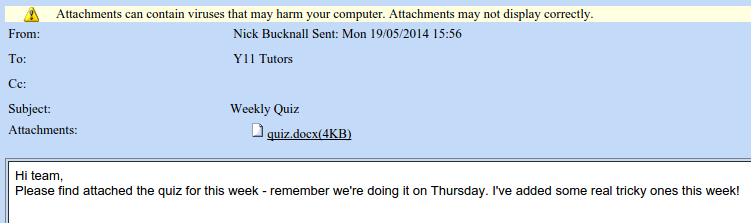
\includegraphics[scale=0.46]{analysis/current_solution/document_inspections/email}
  \caption{Email sent by Nick Bucknall on the 19th May 2014}
\end{figure}

This capture of an email sent by Nick Bucknall (a head of year, soon to be head of house) to his tutor team demonstrates the inefficiency with which the quiz system is currently handled. Sending an email with an attachment once a week is an approach fraught with issues, the most glaring of which is the shocking lack of organisation. As can be gleaned from the shot, the school's email system is not the most modern, and this can make it difficult to find particular emails - such as the weekly quiz. A far better solution would be to have the correct quiz appear automatically.
\clearpage
% subsubsection weekly_email (end)

\subsubsection{Weekly Quiz} % (fold)
\label{ssub:weekly_quiz}
\begin{figure}[h!]
  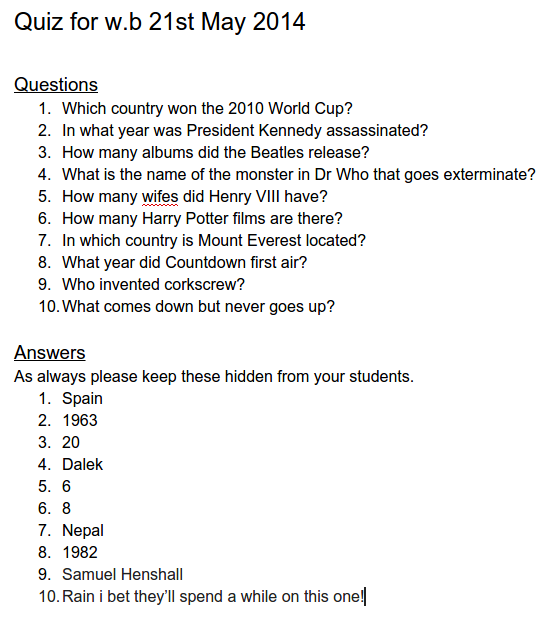
\includegraphics[scale=0.55]{analysis/current_solution/document_inspections/quiz_sample}
  \caption{Quiz created by Nick Bucknall on the 14th May 2014}
\end{figure}

The above capture of a quiz created by Nick Bucknall, and distributed to form tutors, demonstrates the form that that the quizzes currently take. As can be discerned, though the current method undoubtedly works, the existence of the answers so close to the questions causes a number of difficulties; most notably, it means that the questions must be read out by the form tutor, and the actual question sheet cannot be shown. Additionally, it no doubt takes time for Nick Bucknall to lay out the document in such a manner each week; a better solution would be if a standard template could be used (though not, it should be noted, in the form of another word processed document).
\clearpage
% subsubsection weekly_quiz (end)



% Import similar systems
\subsection{Similar Systems}
There are a number of systems available, both free and at a cost, that would allow the school to improve their current method of quiztribution (\textit{quiz distribution}). Several popular options are outlined below.

\subsubsection{Quiz Creation Websites}
A number of websites exist that allow users to design, play and share their own quizzes. These websites, including \textit{QuizWorks}, \textit{ExamTime} and \textit{QuizBean} generally follow the same pattern: the user creates an account, is directed to an interface wherein they can design a quiz, and is then given a link with which they can share the quiz with others. For basic quiz creation, these websites are free, though for more advanced usage (\textit{QuizWorks} defines an ``advanced'' quiz as one containing more than 15 questions), paid plans are available.

As these systems are websites, they can be accessed from practically any computer or mobile device, as long as there is an internet connection in range. This means that users can continue to work on their quizzes, whether designing or answering them, outside of their place of work.

Though these systems are undoubtedly useful, and could, with a few compromises, be easily integrated into the school's routines, they lack an awareness of the structure of a school. There is no concept of ``form groups'' or ``heads of year'', both are which are vital concepts if the system is to meet what the school desires. Additionally, they lack the ability to display a detailed analysis of the results (at least, not without paying a somewhat exorbitant fee - \pounds60 per month in the case of \textit{QuizWorks}), a side effect of their focus on individuals as opposed to groups.

\subsubsection{Quiz Creation Software Packages}
Similar to quiz creation websites, quiz creation software packages allow the user to design and play a quiz. However, these systems are desktop applications (the majority are designed for Microsoft Windows), and so can only be accessed from a single desktop or laptop system. Examples of these systems include \textit{Wondershare Quiz Creator}, \textit{Tanida QuizBuilder}, and \textit{Articulate Storyline 2}. Unlike the mostly free websites, these software packages are often very expensive: the three systems mentioned range in price from \$99 - \$1846 for a single license, with additional licenses costing even more.

To compensate for the high prices, these desktop applications contain a vast feature set. Quizzes of every imaginable type can be created, from drag-and-drop, multiple choice, word bank quizzes, and many more. Images can be included, points assigned, and complex animations can be set to make the quiz as visually appealing as possible. In addition, reports can be generated with tremendous amounts of data, showcasing practically every data point imaginable.

Useful though these features are, they are a touch overkill for what the school's purposes. The systems are not the easiest things to use in the world, something that, considering the teacher's relative lack of IT skills, is quite a drawback. Additionally, the high costs make the systems prohibitively expensive, considering the school's status as the worst funded school in the county.

\subsubsection{Quizdom}

% Import justification of methods
\subsection{Justification of Methods}

Methods will be justified soon.

% Import IPSO chart
\subsection{IPSO Chart}
This IPSO chart describes the inputs, outputs, storage locations and general processes that are associated with the system.

\begin{table}[h]
\centering
\begin{tabular}{|l|l|}
\hline
\multicolumn{1}{|c|}{{\bf Inputs}}                                                                                                                              & \multicolumn{1}{c|}{{\bf Processes}}                                                                                                                                                                                                                                                                         \\ \hline
\begin{tabular}[c]{@{}l@{}}Full name\\ Password\\ \\ Form name\\ \\ Quiz title\\ Quiz questions\\ Quiz answers\\ Forms the quiz should be sent to.\end{tabular} & \begin{tabular}[c]{@{}l@{}}Create HOY accounts from inputs\\ Create form group accounts\\ \\ Create and store quizzes\\ \\ Allow quizzes to be answered by\\ forms and store answers.\\ \\ Prevent quizzes from starting unless\\ all forms have joined.\\ \\ Mark quizzes and analyse results.\end{tabular} \\ \hline
\multicolumn{1}{|c|}{{\bf Storage}}                                                                                                                             & \multicolumn{1}{c|}{{\bf Outputs}}                                                                                                                                                                                                                                                                           \\ \hline
\begin{tabular}[c]{@{}l@{}}Store user accounts\\ Store individual quizzes with answers.\\ Store mark for quizzes.\\ Store analysis of results.\end{tabular}     & \begin{tabular}[c]{@{}l@{}}Quiz containing questions and answers.\\ Analysis of quiz results.\end{tabular}                                                                                                                                                                                                   \\ \hline
\end{tabular}
\caption{IPSO Chart}
\label{my-label}
\end{table}

% Import limitations of current system
\subsection{Limitations of Current System}
There are evidently a large number of issues with the above method. Firstly, distributing the quizzes via a word-processed document is not a particularly efficient method. It results in the network drive being cluttered with a variety of documents, perhaps with a non-existent naming scheme. This makes it harder for the form tutors to find the correct quiz for the week, slowing the whole process down. A more effective solution would be to have everything in it's own self contained system, with its own dedicated quiz screen, which points out the correct quiz to the tutors.

Additionally, having the questions and possible answers on the same document puts the integrity of the quiz at risk. Currently, form tutors get around this by hiding the document, but this can cause complications where students forget the possible answers, as well as other issues. It word be far more effective to always have the quiz displayed on screen on the interactive whiteboard, but the current system prohibits this.

Often, teachers forget about the quiz altogether, or believe it to be on a different date than when it is actually scheduled. This is a relatively common occurrence, and means that the quiz either has to be rescheduled (which those tutors who did remember find annoying), or that particular form has to miss out on the quiz that week; this can damage their overall reputation in the school community. A dedicated system could provide them a notification, perhaps via an email, that they should hold the quiz that afternoon. Additionally, the system could be set up in such a way that the quiz only begins once all the appropriate forms have connected.

Furthermore, the current system is not particularly fair. Students can spend as long as they wish on a single question, as long as the quiz is completed within the 25 minutes given to the form time. It would be fairer if the form was given a time limit of, say 60 seconds, after which the system automatically moves on to the next quiz.

The current system is also very isolated. Following the appointment of the new principal, the school has sought to implement the principle of ``togetherness'', whereby students work together more often. Though the current quiz system aligns itself with this philosophy to a degree (each form works together to come up with the answer), it could be improved by allowing a degree of interoperability between the forms. For example, if a quiz was being answered by all the forms in Year 8, one form could be given the opportunity to pose a question to the other forms, perhaps referencing one of the jokes sanctioned by the school.

By allowing the form tutors themselves to mark the quiz, their is a large risk of
inaccurate results being reported back, possibly altered in such a way that favours the form. Though this allows the head of year to display trust to his team of form tutors, there exists in the school a very competitive atmosphere, increasing the chance that such malpractice will occur. A safer approach would be to allow the system to mark the form's answers, and then report this directly to the head of year.

Though the heads of year throughout the school possess many fine and admirable qualities, it would be remiss to apply to them the label of ``mathematician''.  For simply calculating the best and worst performing forms for any given quiz, there are few issues with the current system (though it would be convenient if this was worked out automatically). It is when attempting to work out more complex results, such as the average score of a form over a period of several years, that the humble head of year falls short. A dedicated system would be able to perform a complicated analysis on the entire set of data it collects, allowing for a far more interesting report to be generated. This data could then be presented at an end of year, or even school, assembly, showcasing the best form in each category (or some other arbitrary statistic) throughout their entire school career.

Finally, the fact that the school is completely replacing the head of year system with new heads of house means that the entire approach
